\section{Facade} 

\subsection{Architecture overview}

Since most of the operations include the interaction with both web3funcions and IPFS packages, we provide a third package, facade, with the aim of hiding the web3 and IPFS layers. This package executes function calls, in the suitable order, to the other two packages, saving and retrieving data from both IPFS and Ethereum.

\begin{figure}[h]
	\centering
	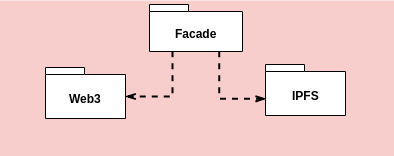
\includegraphics[scale=0.6]{res/images/facade.png}
	\caption{Package diagram with the interaction between facade-web3-IPFS}
\end{figure}

\subsection{Methods}

All the methods describe in the picture below consists of two different steps:
\begin{itemize}
	\item \textbf{setter}: firstly the data is stored to IPFS, then it is stored to Ethereum with related IPFS CID;
	\item \textbf{getter}: firstly the IPFS CID is retrived from web3. The CID is then used to get the 
\end{itemize}
\begin{figure}[H]
	\centering
	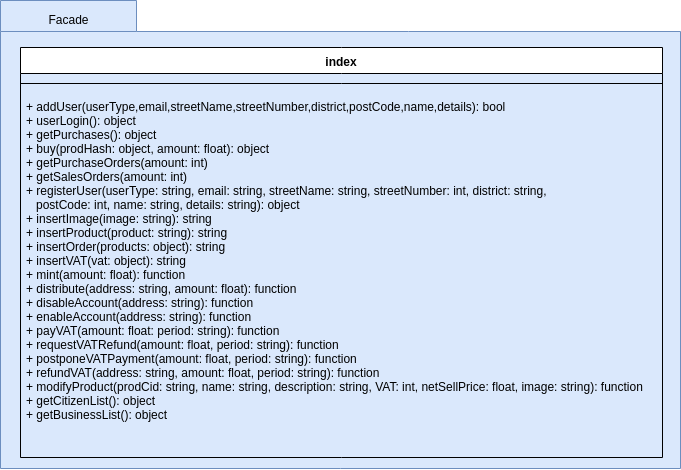
\includegraphics[scale=0.55]{res/images/facade-package.png}
	\caption{Class diagram of the facade package}
\end{figure}

\noindent Since the methods are just a combination of the already described methods of the web3 and IPFS packages, we omit their description.

